\documentclass{beamer}
%\documentclass[xcolor=dvipsnames]{beamer}
\usepackage[english]{babel}
\usepackage[utf8]{inputenc}
\usepackage{graphicx}

\newcommand{\beamer}{\textsc{beamer}}
\newtheorem{definicion}{Definición}
\newtheorem{ejemplo}{Ejemplo}

%%%%%%%%%%%%%%%%%%%%%%%%%%%%%%%%%%%%%%%%%%%%%%%%%%%%%%%%%%%%%%%%%%%%%%%%%%%%%%%
\title[Peresentacion de la asignatura CA ]{Solving simulation optimization problems on grid
computing systems}
\author[Autor]{YOUSEF RAJAEI TABRIZI}
\institute[ULL]{Universidad de La Laguna}
\date[11-1-2016]{\today}
%%%%%%%%%%%%%%%%%%%%%%%%%%%%%%%%%%%%%%%%%%%%%%%%%%%%%%%%%%%%%%%%%%%%%%%%%%%%%%%

\usetheme{Madrid}

%%%%%%%%%%%%%%%%%%%%%%%%%%%%%%%%%%%%%%%%%%%%%%%%%%%%%%%%%%%%%%%%%%%%%%%%%%%%%%%
\definecolor{pantone254}{RGB}{122,59,122}
\definecolor{pantone3015}{RGB}{0,88,147}
\definecolor{pantone432}{RGB}{56,61,66}
\setbeamercolor*{palette primary}{use=structure,fg=white,bg=pantone254}
\setbeamercolor*{palette secondary}{use=structure,fg=white,bg=pantone3015}
\setbeamercolor*{palette tertiary}{use=structure,fg=white,bg=pantone432}
\setbeamercolor*{palette sidebar primary}{use=structure,fg=pantone254}
\setbeamercolor*{palette sidebar tertiary}{use=structure,fg=pantone3015}
\setbeamercolor*{block title}{bg=pantone3015,fg=white}
\setbeamercolor*{alerted text}{fg=pantone432}
\setbeamercolor*{item projected}{fg=pantone254}
\setbeamercolor*{section in toc shaded}{use=structure,fg=structure.fg}
\setbeamercolor*{section in toc}{fg=pantone3015}
\setbeamercolor*{subsection in toc shaded}{fg=pantone3015}
\setbeamercolor*{subsection in toc}{fg=pantone432}

%%%%%%%%%%%%%%%%%%%%%%%%%%%%%%%%%%%%%%%%%%%%%%%%%%%%%%%%%%%%%%%%%%%%%%%%%%%%%%%
\begin{document}
  
%++++++++++++++++++++++++++++++++++++++++++++++++++++++++++++++++++++++++++++++  
\begin{frame}

  \includegraphics[width=0.15\textwidth]{img/ullesc.eps}
  \hspace*{7.5cm}
  \includegraphics[width=0.16\textwidth]{img/etsii.eps}
  \titlepage

  \begin{scriptsize}
    \begin{center}
     Escuela Superior de Ingeniería y Tecnología \\
     Universidad de La Laguna
    \end{center}
  \end{scriptsize}

\end{frame}
%++++++++++++++++++++++++++++++++++++++++++++++++++++++++++++++++++++++++++++++  
%""""""""""""""""""""""""""""""""""""""""""""""""""""""""""""""""""""""""""""""
%""""""""""""""""""""""""""""""""""""""""""""""""""""""""""""""""""""""""""""""
\begin{frame}
\frametitle{Diagramas of expriments }
%------------------------------------------------------------------------------
\begin{figure}[!th]
\begin{center}
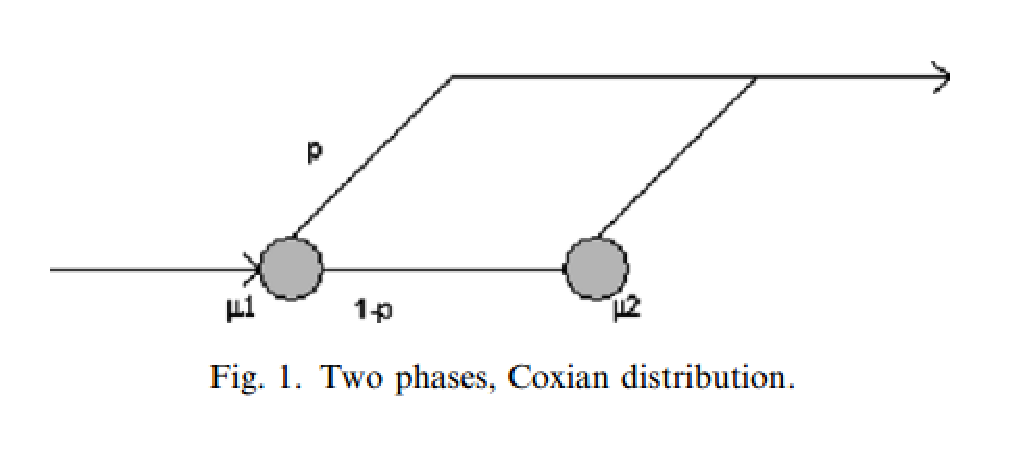
\includegraphics[width=0.75\textwidth]{img/queu.eps}
\caption{frequencia de la aparecion de los barcos}
\label{fig:1}
\end{center}
\end{figure}
%------------------------------------------------------------------------------
\end{frame}
%""""""""""""""""""""""""""""""""""""""""""""""""""""""""""""""""""""""""""""""
%""""""""""""""""""""""""""""""""""""""""""""""""""""""""""""""""""""""""""""""

%++++++++++++++++++++++++++++++++++++++++++++++++++++++++++++++++++++++++++++++  
\begin{frame}
  \frametitle{Índice}  
  \tableofcontents[pausesections]
\end{frame}
%++++++++++++++++++++++++++++++++++++++++++++++++++++++++++++++++++++++++++++++  


\section{Motivación y Objetivos}


%++++++++++++++++++++++++++++++++++++++++++++++++++++++++++++++++++++++++++++++  
\begin{frame}

\frametitle{Motivación}

\begin{definicion}
The optimal assignment of berth slots and cranes to shipping services is the central logistics problem at modern marine
container terminals and should be formulated to specifically account for its stochastic nature. We use a computational grid
to solve a major seaport logistic problem by a simulation optimization approach centred around a queuing network model
of the logistic process of interest. We emphasize the power of grid computing for the simulation optimization studies and
we design and implement an algorithm for distributing the computational load to parallel processors. Performance of the
algorithm is demonstrated numerically using real-sized problem instances.
 2006 Elsevier B.V. All rights reserved.
\end{definicion}

\end{frame}
%++++++++++++++++++++++++++++++++++++++++++++++++++++++++++++++++++++++++++++++  

%++++++++++++++++++++++++++++++++++++++++++++++++++++++++++++++++++++++++++++++  
\begin{frame}

\frametitle{Objetivos }

\begin{block}{Ejemplo}
  \begin{itemize}
  \item
   Using technics of simulation for optimization
  \pause

  \item
   Using techincs of parallelization 

  \end{itemize}
\end{block}

\end{frame}
%++++++++++++++++++++++++++++++++++++++++++++++++++++++++++++++++++++++++++++++  

\section{Fundamentos Teóricos}

\begin{frame}
\frametitle{Fundamentos Teóricos}

In the sequel we illustrate the proposed queuing model in which we eliminate some details from the model
description of Legato and Mazza [12] because they are not significant for the purpose of this paper.
We assume that the occurrence of a delay-time spent at roadstead by an incoming vessel, due to lack of
berth slots, is represented as a special case of the phase type Cox’s distribution. This assumption can be
accepted for the following considerations. Usually, an incoming vessel receives almost immediately the
required slots for berthing. In this case, with a very high probability (p), the elapsing interval from ‘‘arrival
to port’’ and ‘‘berthing time completion’’ results in a very short time (l1, on average), due to the relatively
fast operations for vessel positioning along the berth. With a very low probability (1  p), an arrived vessel
is delayed at roadstead due to unavailability of the required berth slots: once this happens, then a very long
interval (l1 + l2, on average) elapses from ‘‘arrival to port’’ and ‘‘berthing time’’ (Fig. 1).


\end{frame}
%++++++++++++++++++++++++++++++++++++++++++++++++++++++++++++++++++++++++++++++  

\section{Procedimiento experimental}

\begin{frame}
\frametitle{Procedimiento experimental}

In this paper, we focus on the case where incoming vessels (customers) belonging to one out of a set of maritime
shipping ‘‘services’’ (customer classes) can be berthed into shared segments of berth. Each berth segment
(out of ‘‘n’’) corresponds to a fixed number of vessel positions for berthing and is equipped with one or several
cranes; in Fig. 3 it is represented as a multi-server queue with a finite number of waiting places. The delay-time
at roadstead, for berth assignment operations, is represented by a single server queue with unlimited waiting
places.
In the berth planning problem, we should answer the following questions:
• how many segments do we organise for active shipping services?
• how many cranes – out of the total, fixed, number of available ones – do we allocate for each of the organised
segments?
• to which segment do we forward incoming vessels, provided that we may base this decision on some suitable
attributes shared by any given subset of the active services?
Answers to these questions are provided by the simulation optimization approach.

\end{frame}
%++++++++++++++++++++++++++++++++++++++++++++++++++++++++++++++++++++++++++++++  
%""""""""""""""""""""""""""""""""""""""""""""""""""""""""""""""""""""""""""""""
%""""""""""""""""""""""""""""""""""""""""""""""""""""""""""""""""""""""""""""""
\begin{frame}
\frametitle{Diagramas of expriments }
%------------------------------------------------------------------------------
\begin{figure}[!th]
\begin{center}
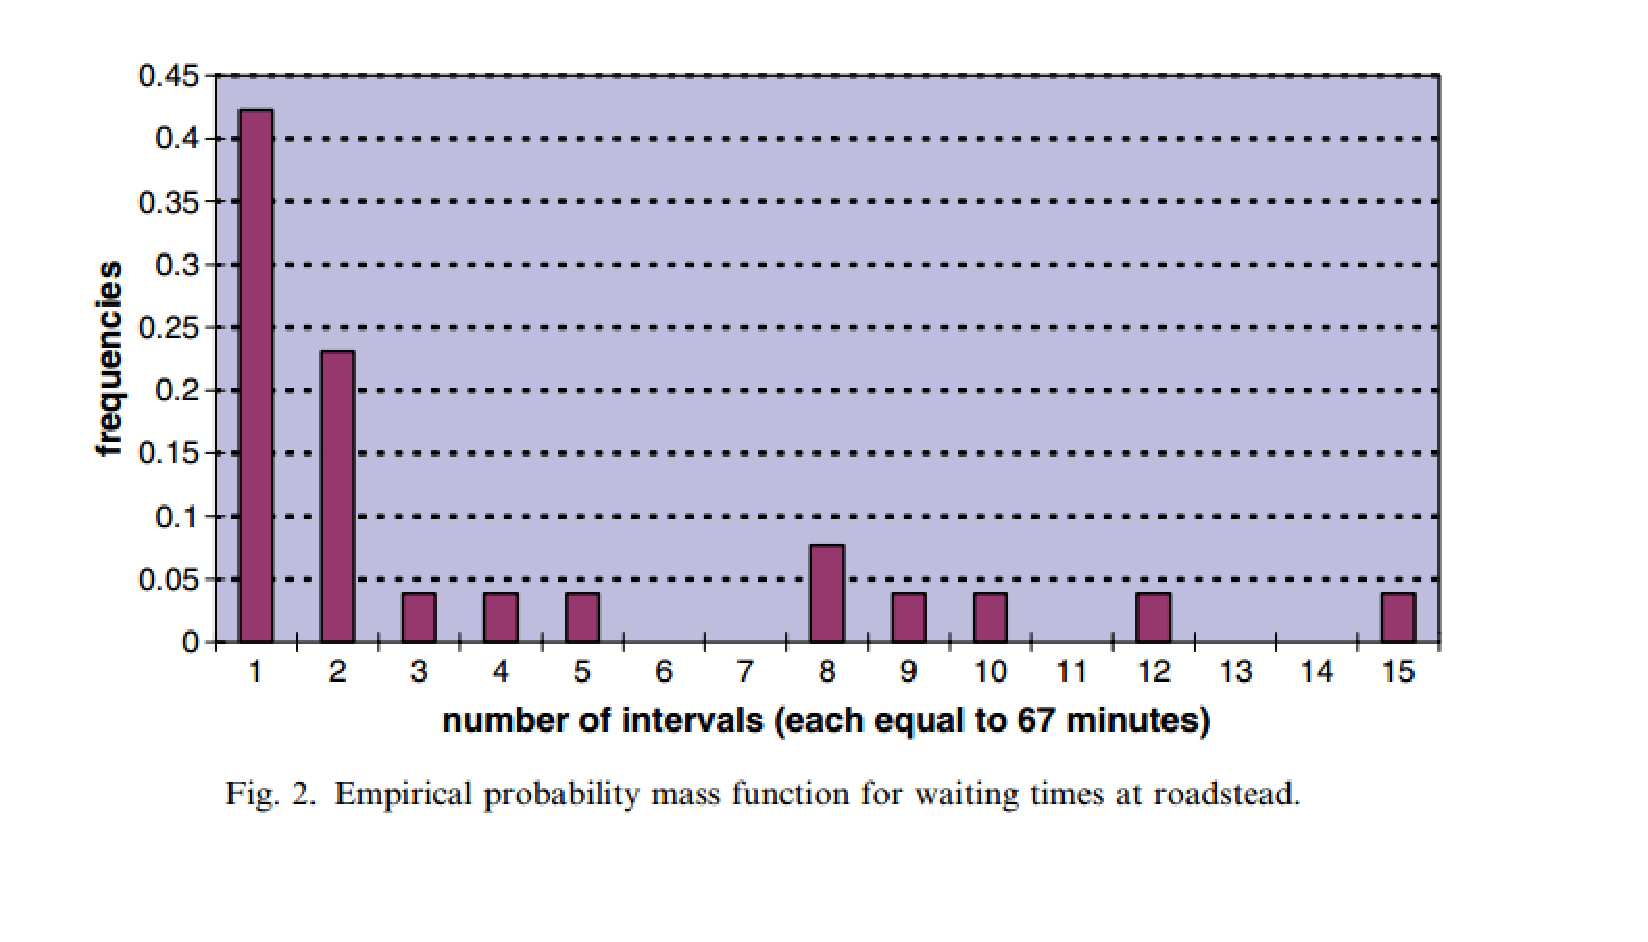
\includegraphics[width=0.75\textwidth]{img/diagrama.eps}
\caption{frequencia de la aparecion de los barcos}
\label{fig:1}
\end{center}
\end{figure}
%------------------------------------------------------------------------------
\end{frame}
%""""""""""""""""""""""""""""""""""""""""""""""""""""""""""""""""""""""""""""""
%""""""""""""""""""""""""""""""""""""""""""""""""""""""""""""""""""""""""""""""
%""""""""""""""""""""""""""""""""""""""""""""""""""""""""""""""""""""""""""""""
%""""""""""""""""""""""""""""""""""""""""""""""""""""""""""""""""""""""""""""""
\begin{frame}
\frametitle{Diagramas of expriments }
%------------------------------------------------------------------------------
\begin{figure}[!th]
\begin{center}
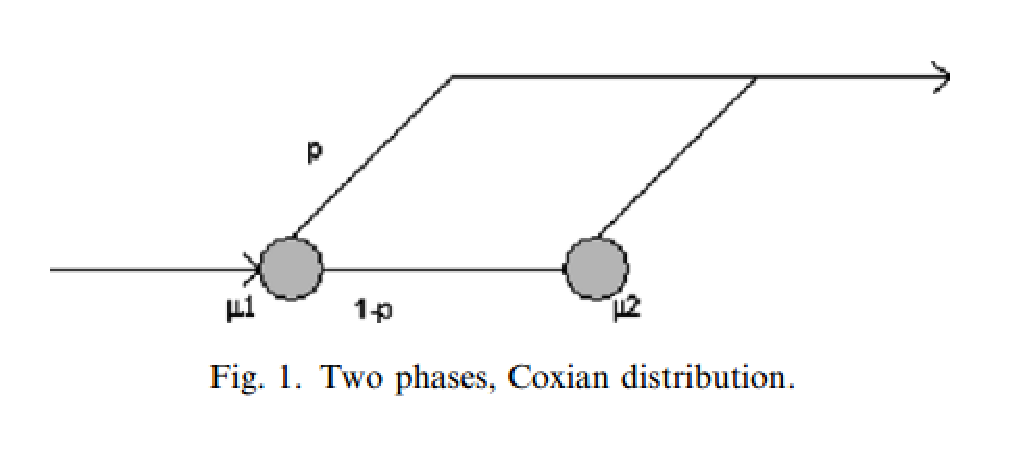
\includegraphics[width=0.75\textwidth]{img/queu.eps}
\caption{frequencia de la aparecion de los barcos}
\label{fig:1}
\end{center}
\end{figure}
%------------------------------------------------------------------------------
\end{frame}
%""""""""""""""""""""""""""""""""""""""""""""""""""""""""""""""""""""""""""""""
%""""""""""""""""""""""""""""""""""""""""""""""""""""""""""""""""""""""""""""""

\subsection{Descripción de los experimentos}

%++++++++++++++++++++++++++++++++++++++++++++++++++++++++++++++++++++++++++++++  
\begin{frame}
\frametitle{A combined procedure for simulation optimization problems}

\begin{ejemplo}
  \begin{itemize}
    \item <1-> Algorithm description 
    \item <2-> Grid enabled versions for the SARP algorithm 
    \item <3> Algorithm 2. SARP 
  \end{itemize}
\end{ejemplo}

\end{frame}
%++++++++++++++++++++++++++++++++++++++++++++++++++++++++++++++++++++++++++++++  

\subsection{Descripción del Algorithms }
%++++++++++++++++++++++++++++++++++++++++++++++++++++++++++++++++++++++++++++++  
\begin{frame}
\frametitle{Hardware y Software}

\begin{ejemplo}
  \begin{enumerate}
    \item
      With the aim of developing grid versions of the SARP algorithm described above (in the sequel G-SARP),
we have adopted a master/worker approach [16,4,19].
Let p be the number of workers. At iteration k, the master creates p + 1 perturbations of a same configuration
of the system (i.e. p + 1 neighbours of the current solution), keeps for itself the first generated configuration
to be estimated and sends the others to the workers (one configuration for each worker). Each processor,
including the master, must decide if its own configuration can be accepted or not. If a processor accepts its
own solution (according to the acceptance criterion of SARP), then sends it to the master. If the master has
new solutions to examine, it selects the next configuration, otherwise it keeps the old one. There are different
rules for selection; for example, the master can choose the configuration with the best estimated performance
(best strategy) or it can make a random choice (random strategy). We have implemented both, and we present in 
      \pause

    \item
 Nasim2
  \end{enumerate}
\end{ejemplo}

\end{frame}
%++++++++++++++++++++++++++++++++++++++++++++++++++++++++++++++++++++++++++++++  

\subsection{Resultados obtenidos}
%++++++++++++++++++++++++++++++++++++++++++++++++++++++++++++++++++++++++++++++  
\begin{frame}
\frametitle{Computational experiments}

%------------------------------------------------------------------------------
\input{tables/table.tex}
%------------------------------------------------------------------------------

\end{frame}
%++++++++++++++++++++++++++++++++++++++++++++++++++++++++++++++++++++++++++++++  


\subsection{Análisis de los resultados}
%++++++++++++++++++++++++++++++++++++++++++++++++++++++++++++++++++++++++++++++  
\begin{frame}
\frametitle{Diagramas of expriments }

%------------------------------------------------------------------------------
\begin{figure}[!th]
\begin{center}
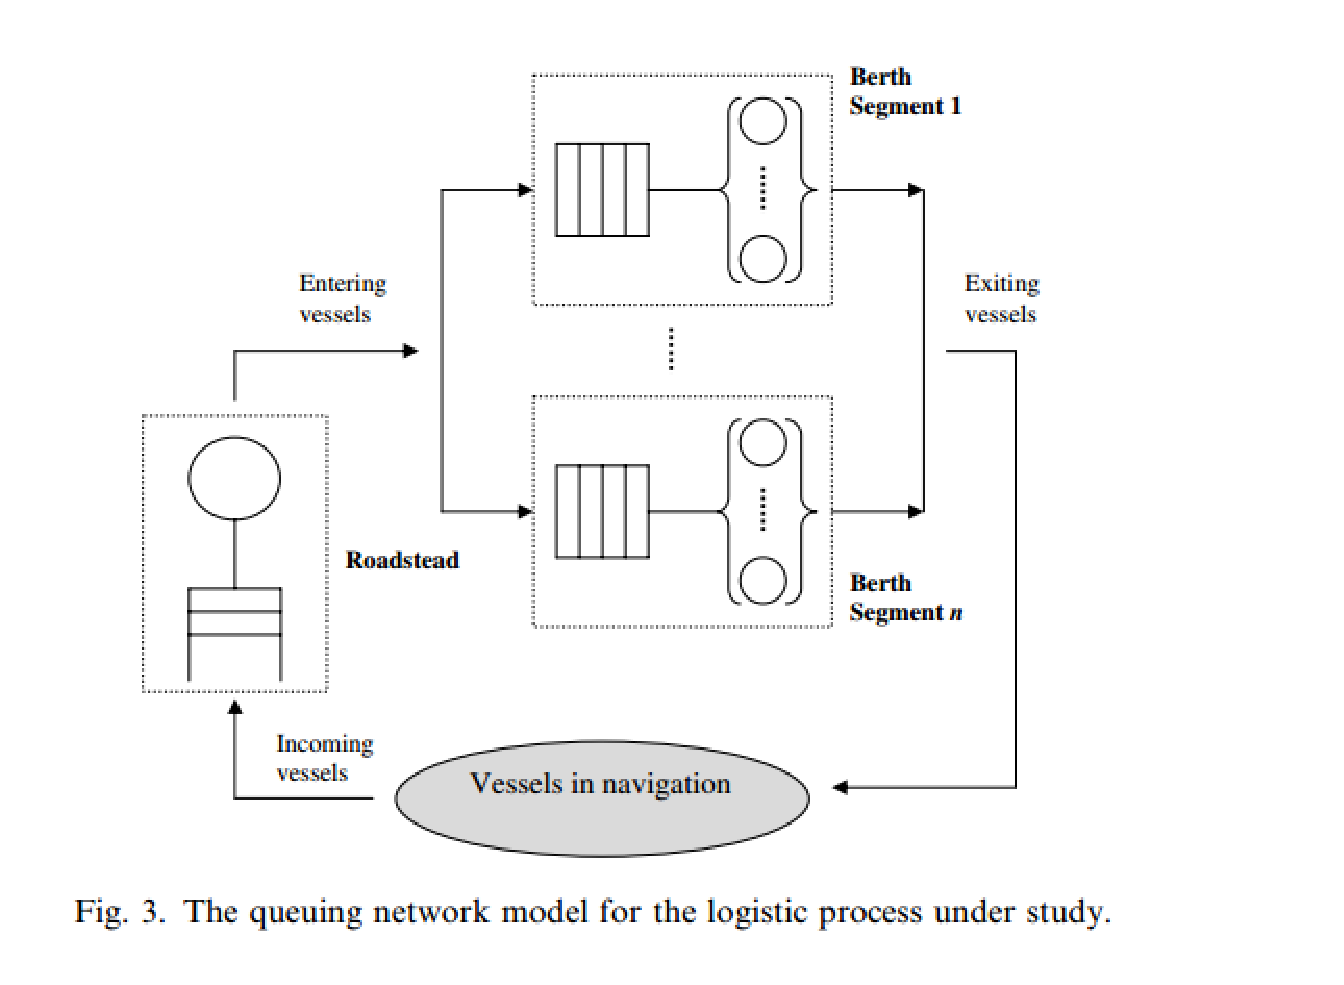
\includegraphics[width=0.75\textwidth]{img/imagen_moeye.eps}
\caption{imagen de la muelle}
\label{fig:1}
\end{center}
\end{figure}
%------------------------------------------------------------------------------

\end{frame}
%++++++++++++++++++++++++++++++++++++++++++++++++++++++++++++++++++++++++++++++  
%""""""""""""""""""""""""""""""""""""""""""""""""""""""""""""""""""""""""""""""
%""""""""""""""""""""""""""""""""""""""""""""""""""""""""""""""""""""""""""""""
\begin{frame}
\frametitle{Diagramas of expriments }
%------------------------------------------------------------------------------
\begin{figure}[!th]
\begin{center}
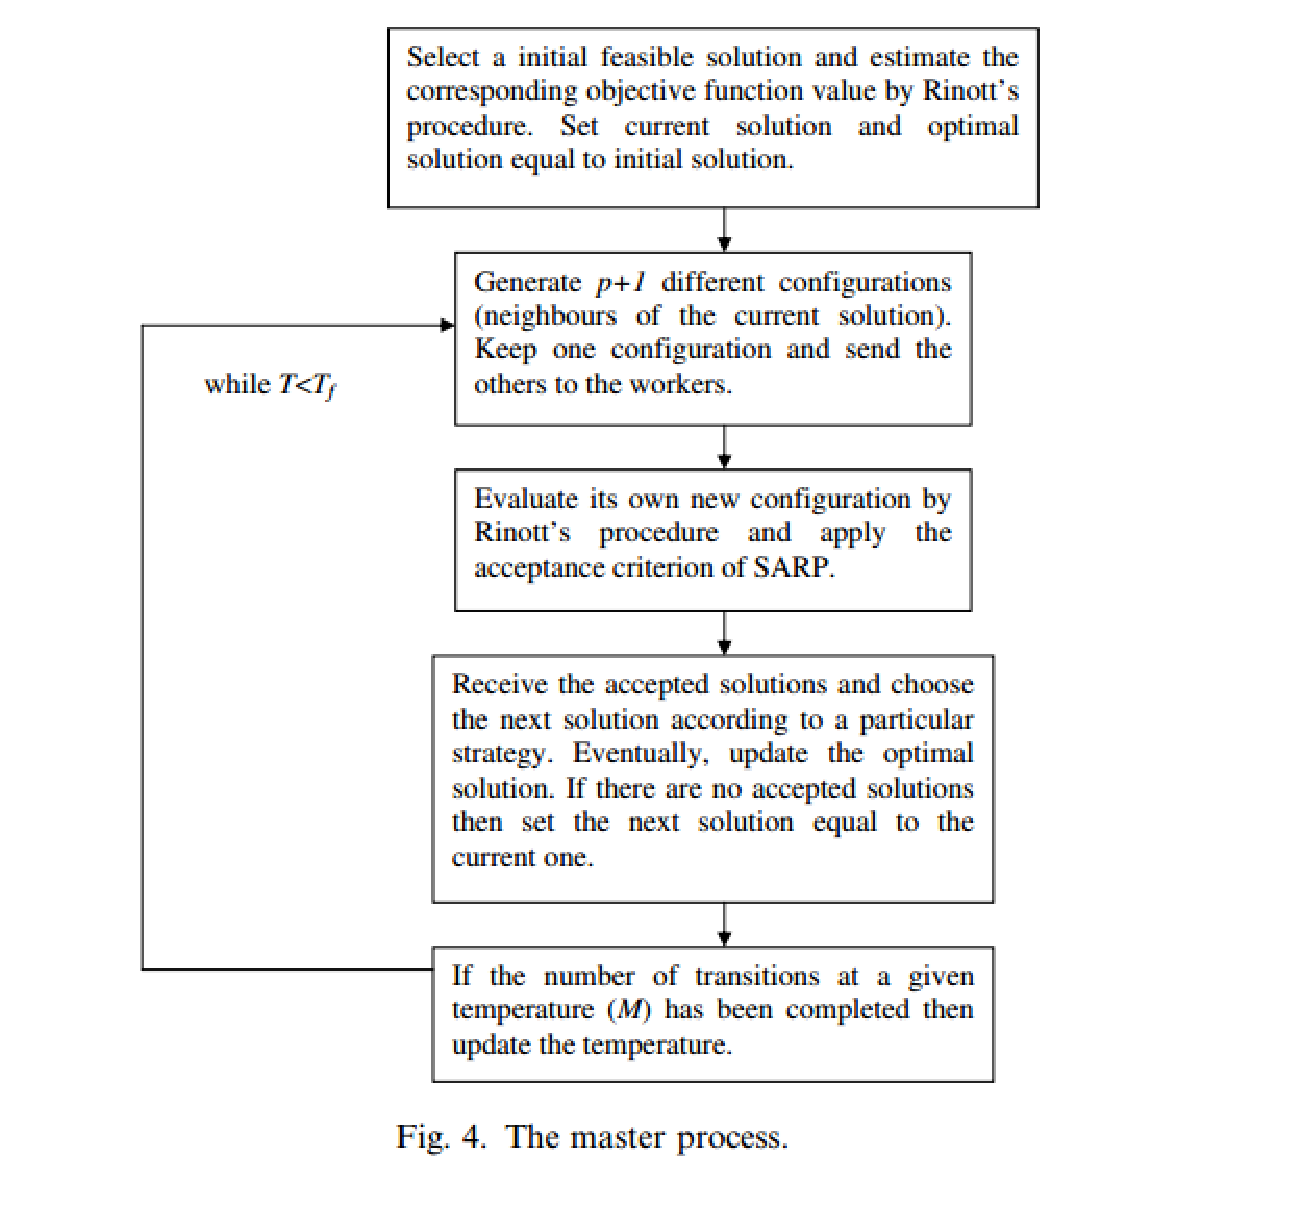
\includegraphics[width=0.75\textwidth]{img/master_p.eps}
\caption{imagen de la muelle}
\label{fig:1}
\end{center}
\end{figure}
%------------------------------------------------------------------------------
\end{frame}
%""""""""""""""""""""""""""""""""""""""""""""""""""""""""""""""""""""""""""""""
%""""""""""""""""""""""""""""""""""""""""""""""""""""""""""""""""""""""""""""""
\section{Conclusiones}

%++++++++++++++++++++++++++++++++++++++++++++++++++++++++++++++++++++++++++++++  
\begin{frame}
\frametitle{Conclusiones}

\begin{ejemplo}
  \begin{enumerate}
    \item
      We have designed and implemented on a grid platform a simulation optimization algorithm that requires a
limited amount of communication and a minimal synchronization among computing resources. It could be
used for a cost-effective solution of logistics decision problems at seaport container terminals. Numerical evidence
shows that as the number of workers increases, the quality of the final solution improves. A crucial role
is played by the optimal compromise between searching the entire feasible region (exploration) and locally
searching promising sub-regions (exploitation).
      \pause
    \item
  Nasim3
  \end{enumerate}
\end{ejemplo}

\end{frame}
%++++++++++++++++++++++++++++++++++++++++++++++++++++++++++++++++++++++++++++++  

%++++++++++++++++++++++++++++++++++++++++++++++++++++++++++++++++++++++++++++++  
\begin{frame}
  \frametitle{Bibliografía}

  \begin{thebibliography}{10}

    \beamertemplatebookbibitems
    \bibitem[URL: CTAN]{latex} 
    CTAN. {\small $http://www.ctan.org/$}

    \beamertemplatebookbibitems
    \bibitem[Tantau, 2005]{beamer} 
    Tantau, Till. 
    \emph{User's Guide to the \beamer{} Class, Version 3.06, 2005} 
    {\small $http://ctang.tug.org/tex-archive/macros/latex/contrib/beamer$}


  \end{thebibliography}
\end{frame}


%++++++++++++++++++++++++++++++++++++++++++++++++++++++++++++++++++++++++++++++  

\end{document}
